% ---------------------------------------------------------------------------
%  Generated by gen_tikz.py; edit that, not this.
% ---------------------------------------------------------------------------
\begin{figure}[H]
\centering
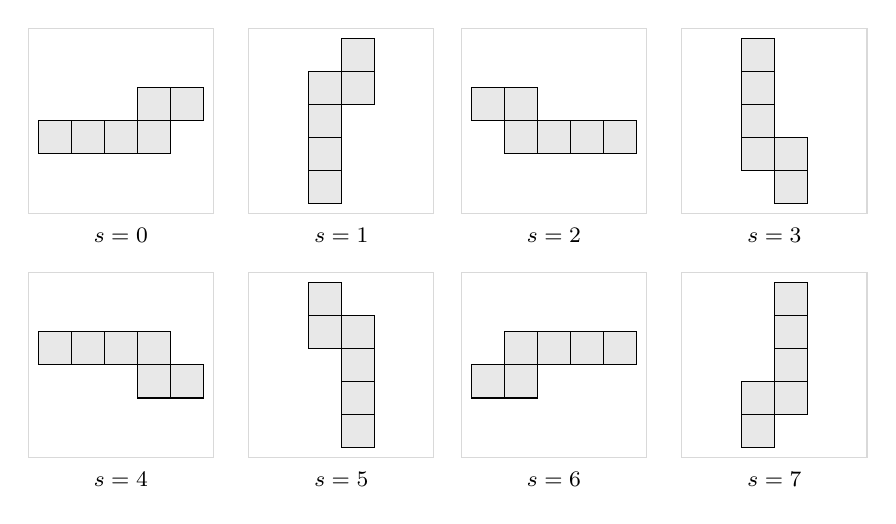
\begin{tikzpicture}[x=4.2mm,y=4.2mm,font=\small]
\begin{scope}[xshift=0.0cm,yshift=0.0cm]
\draw[gray!30] (0,0) rectangle (5.6,5.6);
\filldraw[fill=gray!18] (0.30,1.80) rectangle +(1,1);
\filldraw[fill=gray!18] (1.30,1.80) rectangle +(1,1);
\filldraw[fill=gray!18] (2.30,1.80) rectangle +(1,1);
\filldraw[fill=gray!18] (3.30,1.80) rectangle +(1,1);
\filldraw[fill=gray!18] (3.30,2.80) rectangle +(1,1);
\filldraw[fill=gray!18] (4.30,2.80) rectangle +(1,1);
\node[below,font=\footnotesize] at (2.8,-.15) {$s=0$};
\end{scope}
\begin{scope}[xshift=2.8cm,yshift=0.0cm]
\draw[gray!30] (0,0) rectangle (5.6,5.6);
\filldraw[fill=gray!18] (1.80,0.30) rectangle +(1,1);
\filldraw[fill=gray!18] (1.80,1.30) rectangle +(1,1);
\filldraw[fill=gray!18] (1.80,2.30) rectangle +(1,1);
\filldraw[fill=gray!18] (1.80,3.30) rectangle +(1,1);
\filldraw[fill=gray!18] (2.80,3.30) rectangle +(1,1);
\filldraw[fill=gray!18] (2.80,4.30) rectangle +(1,1);
\node[below,font=\footnotesize] at (2.8,-.15) {$s=1$};
\end{scope}
\begin{scope}[xshift=5.5cm,yshift=0.0cm]
\draw[gray!30] (0,0) rectangle (5.6,5.6);
\filldraw[fill=gray!18] (0.30,2.80) rectangle +(1,1);
\filldraw[fill=gray!18] (1.30,1.80) rectangle +(1,1);
\filldraw[fill=gray!18] (1.30,2.80) rectangle +(1,1);
\filldraw[fill=gray!18] (2.30,1.80) rectangle +(1,1);
\filldraw[fill=gray!18] (3.30,1.80) rectangle +(1,1);
\filldraw[fill=gray!18] (4.30,1.80) rectangle +(1,1);
\node[below,font=\footnotesize] at (2.8,-.15) {$s=2$};
\end{scope}
\begin{scope}[xshift=8.3cm,yshift=0.0cm]
\draw[gray!30] (0,0) rectangle (5.6,5.6);
\filldraw[fill=gray!18] (1.80,1.30) rectangle +(1,1);
\filldraw[fill=gray!18] (1.80,2.30) rectangle +(1,1);
\filldraw[fill=gray!18] (1.80,3.30) rectangle +(1,1);
\filldraw[fill=gray!18] (1.80,4.30) rectangle +(1,1);
\filldraw[fill=gray!18] (2.80,0.30) rectangle +(1,1);
\filldraw[fill=gray!18] (2.80,1.30) rectangle +(1,1);
\node[below,font=\footnotesize] at (2.8,-.15) {$s=3$};
\end{scope}
\begin{scope}[xshift=0.0cm,yshift=-3.1cm]
\draw[gray!30] (0,0) rectangle (5.6,5.6);
\filldraw[fill=gray!18] (0.30,2.80) rectangle +(1,1);
\filldraw[fill=gray!18] (1.30,2.80) rectangle +(1,1);
\filldraw[fill=gray!18] (2.30,2.80) rectangle +(1,1);
\filldraw[fill=gray!18] (3.30,1.80) rectangle +(1,1);
\filldraw[fill=gray!18] (3.30,2.80) rectangle +(1,1);
\filldraw[fill=gray!18] (4.30,1.80) rectangle +(1,1);
\node[below,font=\footnotesize] at (2.8,-.15) {$s=4$};
\end{scope}
\begin{scope}[xshift=2.8cm,yshift=-3.1cm]
\draw[gray!30] (0,0) rectangle (5.6,5.6);
\filldraw[fill=gray!18] (1.80,3.30) rectangle +(1,1);
\filldraw[fill=gray!18] (1.80,4.30) rectangle +(1,1);
\filldraw[fill=gray!18] (2.80,0.30) rectangle +(1,1);
\filldraw[fill=gray!18] (2.80,1.30) rectangle +(1,1);
\filldraw[fill=gray!18] (2.80,2.30) rectangle +(1,1);
\filldraw[fill=gray!18] (2.80,3.30) rectangle +(1,1);
\node[below,font=\footnotesize] at (2.8,-.15) {$s=5$};
\end{scope}
\begin{scope}[xshift=5.5cm,yshift=-3.1cm]
\draw[gray!30] (0,0) rectangle (5.6,5.6);
\filldraw[fill=gray!18] (0.30,1.80) rectangle +(1,1);
\filldraw[fill=gray!18] (1.30,1.80) rectangle +(1,1);
\filldraw[fill=gray!18] (1.30,2.80) rectangle +(1,1);
\filldraw[fill=gray!18] (2.30,2.80) rectangle +(1,1);
\filldraw[fill=gray!18] (3.30,2.80) rectangle +(1,1);
\filldraw[fill=gray!18] (4.30,2.80) rectangle +(1,1);
\node[below,font=\footnotesize] at (2.8,-.15) {$s=6$};
\end{scope}
\begin{scope}[xshift=8.3cm,yshift=-3.1cm]
\draw[gray!30] (0,0) rectangle (5.6,5.6);
\filldraw[fill=gray!18] (1.80,0.30) rectangle +(1,1);
\filldraw[fill=gray!18] (1.80,1.30) rectangle +(1,1);
\filldraw[fill=gray!18] (2.80,1.30) rectangle +(1,1);
\filldraw[fill=gray!18] (2.80,2.30) rectangle +(1,1);
\filldraw[fill=gray!18] (2.80,3.30) rectangle +(1,1);
\filldraw[fill=gray!18] (2.80,4.30) rectangle +(1,1);
\node[below,font=\footnotesize] at (2.8,-.15) {$s=7$};
\end{scope}
\end{tikzpicture}
\caption{The target in its eight allowed orientations, in the codes
$s=0,\dots,7$ that the certificate data use: $s=0$ is $(x,y)$, then $s=1,2,3,4,5,
6,7$ apply $(y,x)$, $(-x,y)$, $(y,-x)$, $(x,-y)$, $(-y,x)$, $(-x,-y)$, $(-y,-x)$.
Every translate of any one of them is a win, so a Maker policy may choose its
orientation in advance and change it later.}
\label{fig:target}
\end{figure}
